\usetikzlibrary{arrows,positioning,shapes.geometric, calc}
\begin{figure}[H]
    \makebox[\textwidth][c]{
        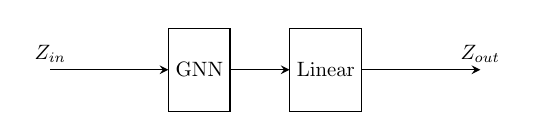
\begin{tikzpicture}[
            >=stealth,
            node distance=4cm,
            block/.style={draw, fill=white, rectangle,
            minimum height=4em},
            sum/.style={draw, fill=white, circle},
            prod/.style={draw, fill=white, circle},
            scale=0.75,
            transform shape
        ]

            \node (input) {};
            \node[block, right=2cm of input, align=center] (gnn) {GNN};
            \node[block, right=1cm of gnn, align=center] (linear) {Linear};

            \node[right=2cm of linear] (output) {};

            \draw[->] (input) -- node[above, pos=0] {$Z_{in} \inrnxfour$} (gnn);
            \draw[->] (gnn) -- (linear);
            \draw[->] (linear) -- node[above, pos=1] {$Z_{out} \inrnxfour$} (output);


        \end{tikzpicture}
    }
    \caption{Any GNN model - a GNN enocder followed by a linear layer.}%
    \label{fig:gnn_model}%
\end{figure}
